\documentclass[10pt]{article}
\usepackage{times} 
\usepackage{fullpage}
\usepackage{hyperref}
\usepackage{graphicx,multirow,xcolor}
\usepackage{float}
\usepackage{fancyvrb}
\usepackage{bussproofs}
\usepackage{booktabs}
\usepackage{amsmath,amssymb,amsthm,latexsym}
\usepackage{listings}
\usepackage{algorithm, algpseudocode}
\usepackage{url}
\usepackage[top=0.5in, bottom=0.5in, left=0.8in, right=0.8in]{geometry}

\newcommand{\ignore}[1]{}
\newcommand{\esubsection}[1]{\vspace{-9pt}\subsection*{#1}\vspace{-7pt}}
\newcommand{\esubsubsection}[1]{\vspace{-7pt}\subsubsection*{#1}\vspace{-5pt}}

\newenvironment{CVerbatim}
 {\singlespacing\center\BVerbatim}
 {\endBVerbatim\endcenter}

\begin{document}
\title{CFL Alias Analysis}
\author{Jia Chen}
\date{\today}
\maketitle

\section{Introduction}

Alias analysis is one of the most important enabling techniques in an optimizing
compiler: without knowing that two pointers cannot alias, performance-critical
compiler optimizations like loop invariant code motion, load/store code motion,
and dead code elimination could not be applied.

Although LLVM uses an IR of partial-SSA form to trivialize the alias analysis of
non-address-taken variables, it still relies on dedicated alias analysis passes
to obtain aliasing information for non-promotable memory
locations~\cite{LLVMAAPage}. Existing alias analyses in LLVM codebase (as of
May 2016) suffers from various issues:
\begin{itemize}
  \item Some analyses, such as basicaa and scev-aa, are intraprocedural and thus
    cannot look beyond function boundaries.
  \item Some analyses are very limited in its scope. For example, globals-aa
    only handles non-address take global variables and simple function
    invocations, while scev-aa only handles aliases in loops.
  \item Some analyses, such as tbaa, rely on the existence of IR metadata to detect
    aliases. If the frontend is not able to emit high-quality metadata, those
    analyses will not be able to produce many useful results.
\end{itemize}

To overcome some of those limitations, a new pass called cfl-aa was added to
LLVM trunk in 2015. The original desgin goal is to have a complement pass
alongside basicaa that
works on all kinds of pointers, does not depend on metadata, and is fast,
more precise, and interprocedural. Before May 2016, some of those goals were
achieved, while some useful features were still missing. Also, due to precision
and stability issues, cfl-aa was never enabled by default in LLVM and clang's production release.

In this year's Google Summer of Code, I worked on a project that aims to bring 
cfl-aa to a usable state. Here is a list of tasks I managed to get done in the
past three months:
\begin{itemize}
  \item Patched various miscompilation bugs in the original cfl-aa. 
  \item Improved analysis precision when handling pointer arithmetics and
    integer casts.
  \item Added a summary-based interprocedure support to cfl-aa.
  \item Added an experimental inclusion-based cfl-aa pass as a more expensive
    but more precise alternative to the current unification-based cfl-aa.
  \item Evaluated how well cfl-aa performs on real-world benchmarks.
  \item Reported 4 different bugs found on other LLVM components.
\end{itemize}

In this article, I will try to explain in more detail what I have
done in the past three months, and where to go next. It also demonstrates the current design and implementation, and
serves as a documentation for those who are interested in
working on cfl-aa in the future.

The rest of this article is organized as follows: background knowledge required
to understand how cfl-aa works is provided in Section~\ref{background}.
Section~\ref{implementation} focuses on how the ideas described in
Section~\ref{background} are implemented. Evaluation of the current
implementaion can be found in Section~\ref{evaluation}. Section~\ref{limitation}
mainly discuss the limitations of the current system
and provide suggestions on how to fix them. Section~\ref{conclusion} concludes
the article.

\section{Background}\label{background}

\subsection{Program Representation}
We starts the discussion by formulating the problem of alias analysis. The input
to the analysis is a program represented in LLVM IR form. For the purpose of
alias analysis, only values of pointer types are of interest to us\footnote{For
  simplicity, pointer-to-integer and integer-to-pointer casts are ignored for the rest of the section. We
  will get back to this issue in Section~\ref{attribute}.}. In addition,
existing alias analyses in LLVM (including cfl-aa) are flow-insensitive, which
means that from the analyses' perspective, control flows are simply ignored, and
instructions in a function may be executed in any order any number of times.

To simplify the discussion, we assume that any input LLVM IR given to the alias
analysis gets canonicalized into the following form:

\begin{eqnarray*}
  Module & ::= & Function^{*} \\
  Function & ::= & Instruction^{*} \\
  Instruction & ::= & Pointer = \textbf{alloc} \\
              & | & Pointer = Pointer^\prime \\
              & | & Pointer = \textbf{load } Pointer^\prime \\
              & | & \textbf{store } Pointer, Pointer^\prime \\
              & | & Pointer = \textbf{call } Function\ (Variable^{*}) \\
              & | & \textbf{return } Pointer
\end{eqnarray*}

An instruction can be a memory allocation (including stack allocation as well as
heap allocation), a pointer assignment, a pointer load/store, or a call/return.
Any LLVM instruction can be either put into one of the six forms, or safely ignored.

\subsection{Alias Analysis and CFL Reachability}\label{cflintro}

The goal of the alias analysis is to compute alias relations between two
$Pointer$s. In this article we primarily focus on may-analyses, meaning that given two pointers
$p$ and $q$, an alias analysis only need to produce one of two possible responses: either $p$ and
$q$ may alias each other, or they must not alias each other.

A number of approaches have been proposed to solve may-alias analysis problem in
the past two decades. The approach adopted by cfl-aa formulates the problem as a context-free
language (CFL) reachability problem. Given a canonicalized input program, we
first translate it into a graph datastructure called Program Expression
Graph~\cite{Reps:1997} (PEG) in the following way:
\begin{itemize}
  \item Each $Pointer$ becomes a node in the graph.
  \item For each assignment instruction $x = y$, add an edge from node $y$ to node $x$
    with edge label \textbf{A} to the graph (\textbf{A} stands for ``assignment'').
  \item For each load instruction $x = \textbf{load }y$, add an edge from node $y$ to
    node $x$ with edge label \textbf{D} to the graph (\textbf{D} stands for ``dereference'').
  \item For each store instruction $\textbf{store } x, y$, add an adge from node
    $y$ to node $x$ with edge label \textbf{D} to the graph.
  \item How call and return instructions are handled depends on the
    context sensitivity of the analysis. A simple context-insensitive scheme is
    to add an \textbf{A}-edge from each actual parameter to each formal
    parameter, and add an \textbf{A}-edge from each return value to the
    left-hand side of each callsite. We will discuss a more precise scheme later in Section~\ref{interproc}.
  \item Finally, for each \textbf{A}-edge from node $x$ to node $y$, add another edge from
    $y$ to $x$ with label $\overline{\textbf{A}}$, and for each \textbf{D}-edge from
    $x$ to $y$ add another edge from $y$ to $x$ with label $\overline{\textbf{D}}$.
\end{itemize}

After the PEG gets constructed, the problem of finding wheter two pointers $x$
and $y$ are aliases then becomes finding whether there is a path in the PEG from
the node that corresponds to $y$ to the node that corresponds to $x$, under the
condition that the string formed by concatenating all edge labels on the path can be
recognized by the context-free grammar shown in figure~\ref{fig:grammar}~\cite{Zheng:2008}.

\begin{figure}[!ht]
  \begin{eqnarray*}
    \textbf{V} & ::= & \overline{\textbf{F}}\quad\textbf{M}?\quad\textbf{F} \\
    \textbf{M} & ::= & \overline{\textbf{D}}\quad\textbf{V}\quad\textbf{D} \\
    \textbf{F} & ::= & {(\textbf{A}\quad\textbf{M}?)}^{*} \\
    \overline{\textbf{F}} & ::= & {(\textbf{M}?\quad\overline{\textbf{A}})}^{*}
  \end{eqnarray*}
  \caption{Context-free grammar for alias analysis\label{fig:grammar}}
\end{figure}

\section{Implementation}\label{implementation}

\subsection{Overview}

There are two cfl-aa passes that perform CFL Reachability based alias
analysis: one is called cfl-steens-aa, and the other one is cfl-anders-aa. They
are mostly identical but differs in how the CFL Reachability gets computed. The
primary reason for the separation between cfl-steens-aa and cfl-anders-aa is
that they each have their own tradeoff between performance and precision.
Details about their differences can be found in Section~\ref{steens} and Section~\ref{anders}.

Both cfl-aa passes analyze every function separately. Within the function they run in an
eager manner: complete aliasing information for the entire function gets computed
upfront, to ensure that subsequent alias queries can be answered cheaply. Across
function boundaries the analyses adopt a demand-driven strategy. Only when a
client makes alias queries on a function do we compute the aliasing infomration
for that function.

The canonicalization procedure described in Section~\ref{cflintro} is
implemented in a
class called \emph{CFLGraphBuilder}. Source code for the class is located at 
\emph{lib/Analysis/CFLGraph.h}. Both cfl-steens-aa and cfl-anders-aa rely on
it to create the aforementioned PEG datastructure (which is called
\emph{CFLGraph} in our implementation).

\subsection{Steensgaard-Style CFL Reachability}\label{steens}

After CFLGraph is constructed, the next task is to compute pairwise CFL Reachability
relations for all pointers in the given function. This is where cfl-steens-aa
and cfl-anders-aa start to look different from one another. In this section we describe the algorithm
used by cfl-steens-aa first\footnote{Note that I take no credit from what gets
  demonstrated in this section. The interprocedural version of cfl-steens-aa in
  LLVM was 90\% finished before I started the project. Nevertheless, other
  components described in this section, such as the cfl-anders-aa pass and the
  interprocedural extension, are mostly my own work. }, and the one used by cfl-anders-aa is the focus of
the next section. 

It is known in the literature that the problem of computing general CFL
Reachability can be reduced to the problem of computing a dynamic
transitive closure, which is not known to have subcubic
solutions~\cite{Reps:1997}. Even if we only consider the CFL Reachability
problem with a fixed grammar shown in figure~\ref{fig:grammar}, I am still not aware
of any algorithm that can do better than $O(n^2)$, which, in some cases, is
too expensive to be added LLVM's pass pipeline. 

The cfl-steens-aa pass utilizes on a simple observation to drastically improve
the worst-case complexity bound: in figure~\ref{fig:grammar}, if we ignore nonterminal
\textbf{A} and nonterminal $\overline{\textbf{A}}$, then the remaining
grammar essentially describes a \emph{Dyck} language (i.e.\ a language that
only recognized balanced parentheses). If the underlying context-free language is
Dyck, CFL Reachability can be computed in linear (if the corresponding
graph is a tree) or log-linear (if the corresponding graph is more general than
a tree) time, with the right choice of data structure~\cite{Zhang:2013}. 

The way cfl-steens-aa ignores \textbf{A} and $\overline{\textbf{A}}$ is to
perform node merging on CFLGraph: if two nodes on the graph are connected by an
\textbf{A}-edge or an $\overline{\textbf{A}}$-edge, the two will be
collapsed into a single node. We repeat this process until all \textbf{A} and
$\overline{\textbf{A}}$ edges are removed from the graph. Then we apply the
$O(n)$ algorithm proposed in~\cite{Zhang:2013} to compute the Dyck CFL Reachability
of the simplified graph. The algorithm will eventually group pointers into
equivalent sets, and we can tell if two pointers may-alias each other by
checking whether or not they are in the same equivalent set.

The node collapse trick mentioned previously essentially approximate nonterminal
\textbf{V} and nonterminal \textbf{M} in the original grammar by their
transitive closures. It overapproximates the CFL Reachability of the original
grammar, meaning that the analysis could answer
\emph{MayAlias} even if in the original grammer the answer should have been \emph{NoAlias}. In terms of
analysis precision, it has been shown in~\cite{Zheng:2008} that treating \textbf{V} and \textbf{M} as
transitive relations lead to an analysis that is equivalent to Steensgaard's
unification-based algorithm~\cite{Steensgaard:1996}.  

\subsection{Andersen-Style CFL Reachability}\label{anders}

Although cfl-steens-aa successfully brings the cost of CFL Reachability
computation down, it achieves the goal by sacrificing analysis precision.
Consider the following code snippet containing three pointers $x$, $y$ and $z$:
\begin{lstlisting}[escapeinside={/*}{*/}]
  x = /*\textbf{alloc}*/;
  y = /*\textbf{alloc}*/;
  z = x;
  z = y;
\end{lstlisting}

When running cfl-steens-aa on it, all three pointers gets collapsed into the
same node, which means that cfl-steens-aa cannot distinguish them from one
another: the three pointers are treated as pairwise aliases by the
analysis. However, it is obvious from the code that the two pointers $x$ and $y$ should not
alias each other, since they each point to a different memory allocation.

Here is another example:
\begin{lstlisting}[escapeinside={/*}{*/}]
  x = /*\textbf{alloc}*/;
  y = /*\textbf{alloc}*/;
  *a = x;
  *b = y;
  *c = x;
  *c = y;
\end{lstlisting}
If we examine the snippet manually, we can see that pointer $a$ and $b$ do not
alias each other, but both of them alias $c$. But if we feed this program to
cfl-steens-aa, it will try to unify both $(a, b)$ and $(b, c)$, therefore
creating spurious alias pair $(a, c)$. 

Cfl-steens-aa tries to gain analysis speed at the cost of analysis precision. In
contrast, its cousin cfl-anders-aa picks another tradeoff, where precision is valued
over performance. In cfl-anders-aa, the original grammar shown in
figure~\ref{fig:grammar} is used. No overapproximation is performed. The
justification for building cfl-anders-aa is that, although the
theoretical bound to compute CFL Reachability is cubic, in practice the worst-case bound is rarely
hit~\cite{Sridharan:2009}. Also, there has been some evidences that suggest
with the right set of optimization implemented, analyses that are equivalent
to cfl-anders-aa can scale well~\cite{Hardekopf:2007}\cite{Hardekopf:2007_2}.
One additional consideration is that it is often easier for non-unification-based
algorithms to capitalize on field-sensitivity. And finally, even if
cfl-anders-aa never gets practical in terms of performance, it is still worth
implementing just to see how much more precision we can get compared to
cfl-steens-aa. If anyone needs the extra precision, they can always turn it on. 

The algorithm used for cfl-anders-aa comes from existing work~\cite{Zheng:2008}.
The basic idea of the algorithm is to perform a traditional transitive closure
computation to propagate the reachability information, but stop propagating if
it is found that the edge labels do not form a string that can be recognized by
the CFL grammar. To facilitate CFL grammar recognition, the grammar is encoded
using a hierarchical, recursive state machine, and we can tell whether we should
propagate CFL reachability along a given edge by checking if the label on the
edge can direct us from an accepted state in the state
machine to another accepted state. Pseudocode of the algorithm can be found in
Figure~4 of the paper.

Despite the similarity, in cfl-anders-aa we do deviate from the algorithm
described in the paper~\cite{Zheng:2008} in the following two ways. First, our
algorithm eagerly computes all alias pairs after the CFLGraph is built, while in
the paper the authors did the computation in a demand-driven fashion. This is
achieved by initializing the worklist with all neighbors in CFLGraph,
instead of only putting the pair being queried into the worklist. We did not
implement the demand-driven algorithm due to the additional coding complexity
and higher memory profile. Second, in the paper the authors use a state machine
that does not distinguish value reads from value writes. We try to differentiate
the two, as the information of
whether a given pointer is read from or written to turned out to be crucial for
building alias summaries as well as modref summaries. Our implementation ends up using a modified version of
the paper's state machine (shown in figure~\ref{fsm2}), where some states in the original machine (shown in figure~\ref{fsm1}) were
duplicated just to ensure value reads and value writes were not conflated. 

It has been shown that the algorithm we use here is
equivalent to Andersen's inclusion-based algorithm~\cite{Andersen:1994} in terms
of analysis precision.

\begin{figure}
  \centering
  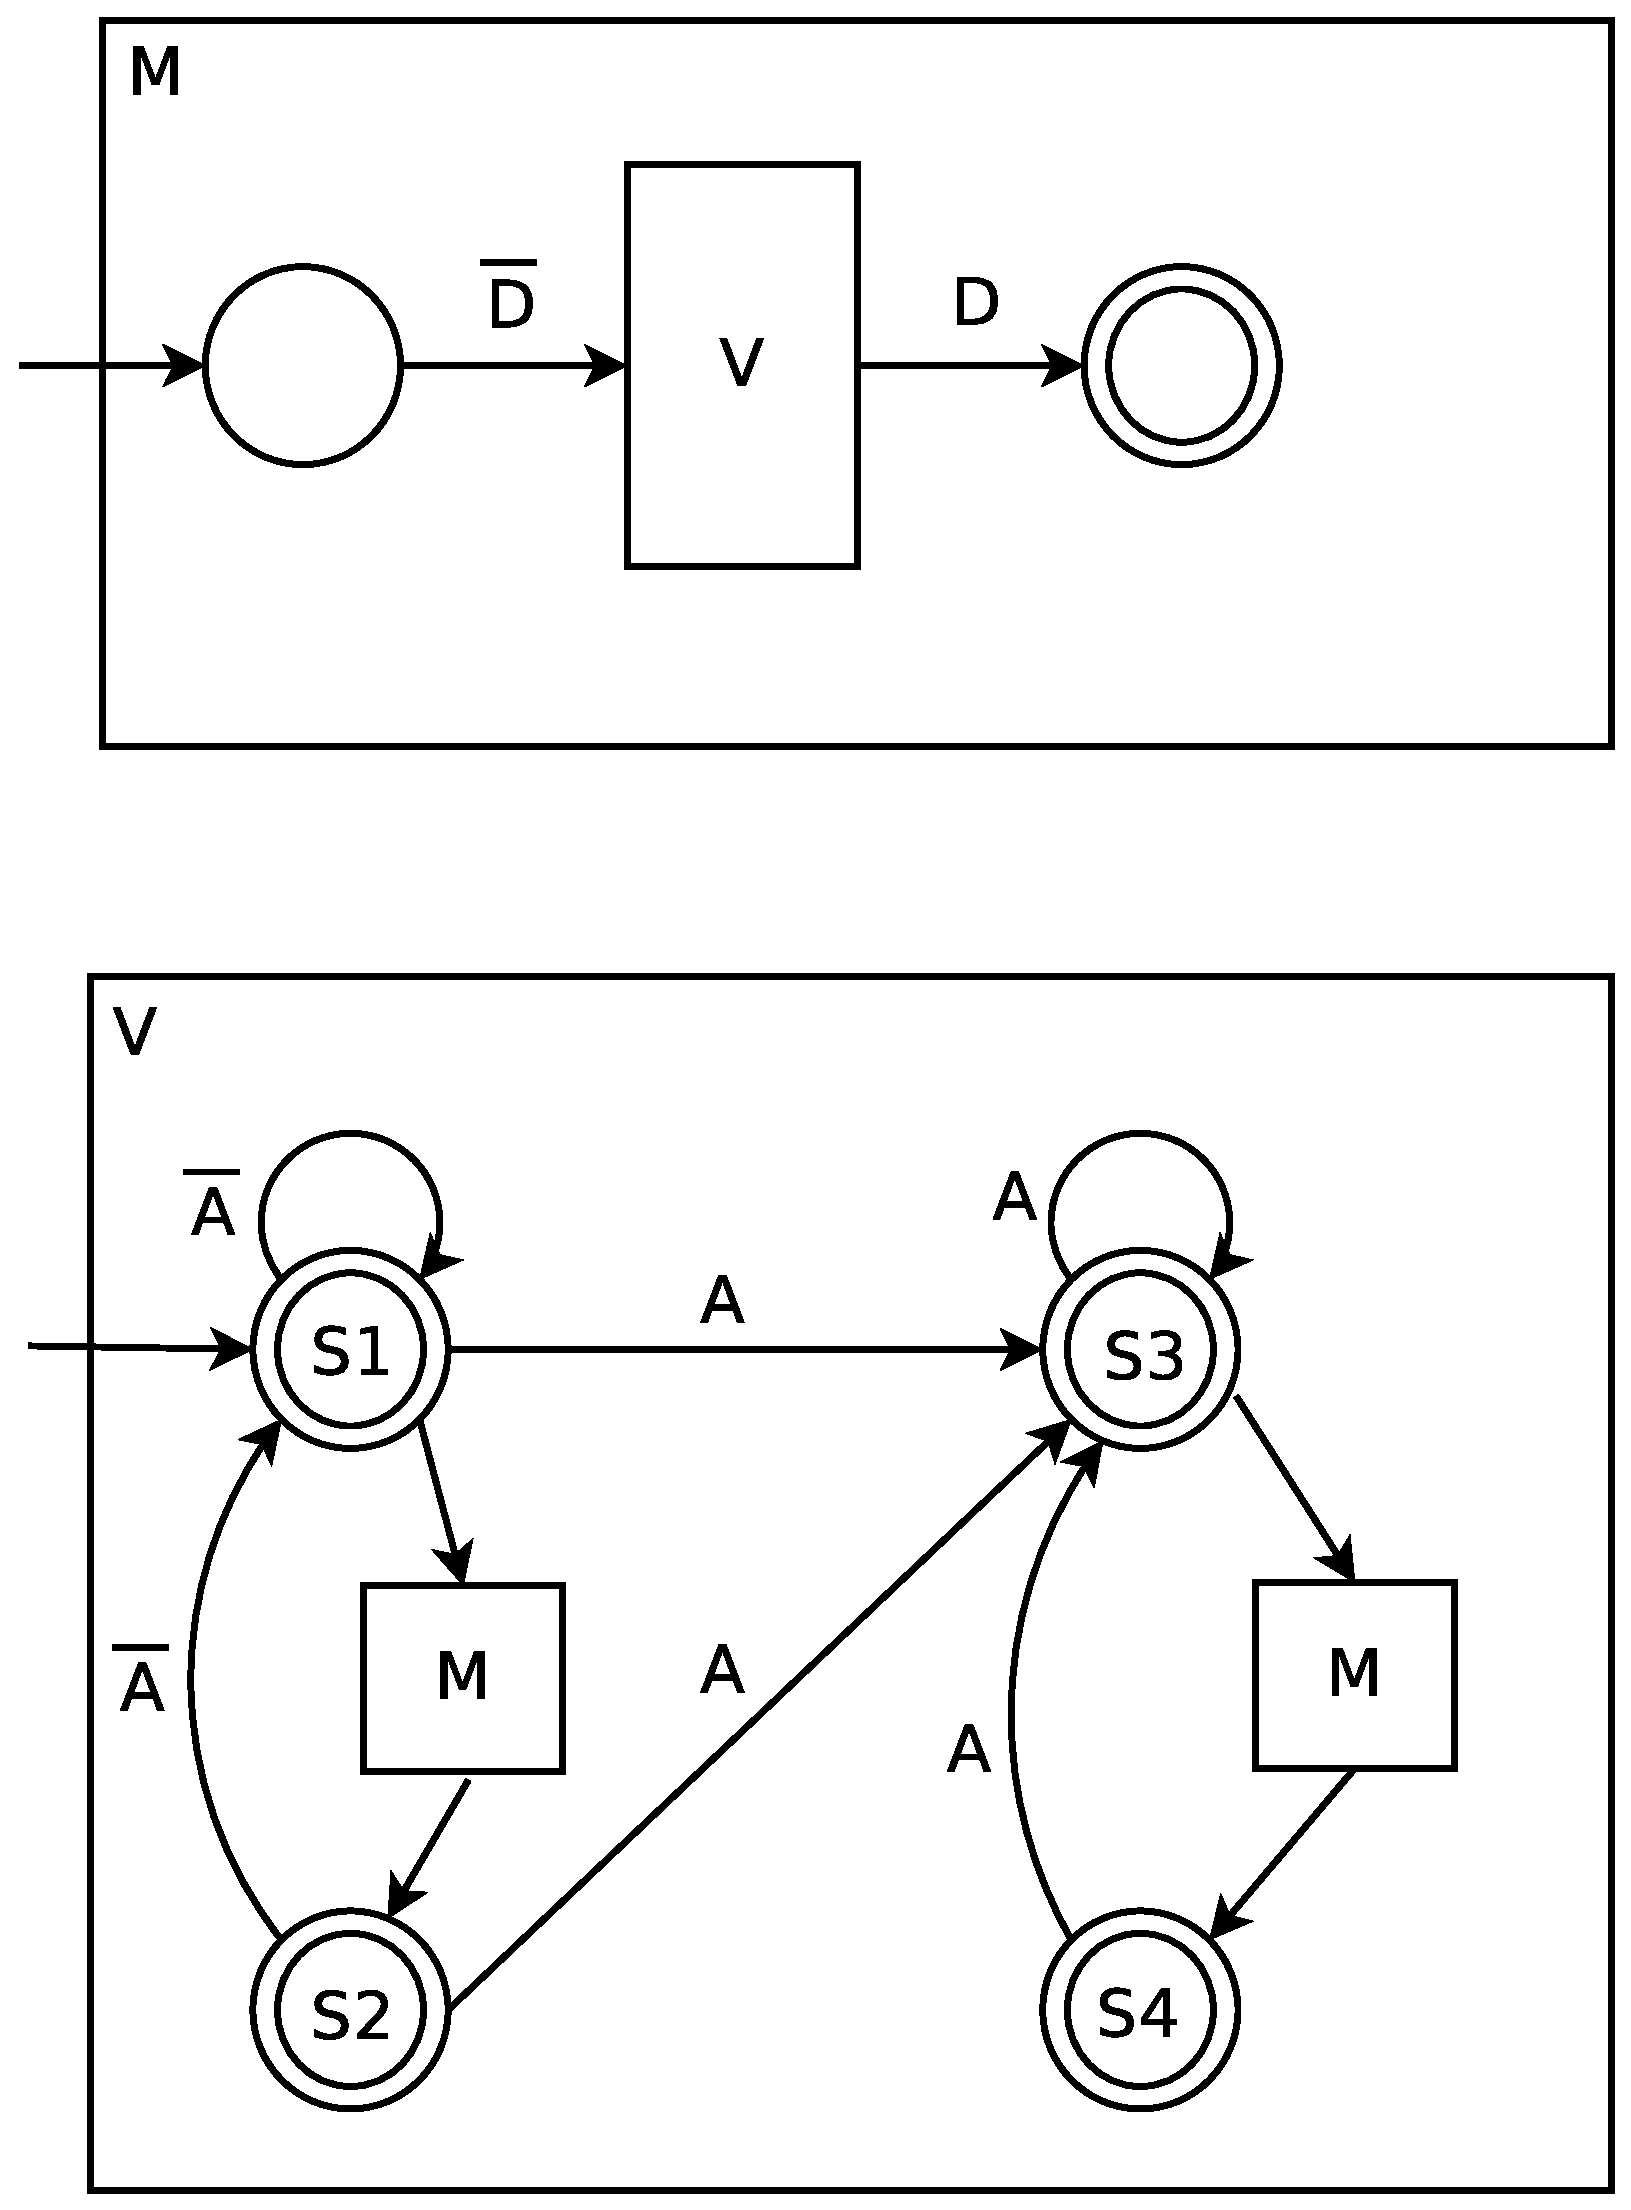
\includegraphics[width=150pt]{FSM1.eps}
  \caption{Hierarchical State Machine used by Zheng et al~\cite{Zheng:2008}.\label{fsm1} }
\end{figure}

\begin{figure}
  \centering
  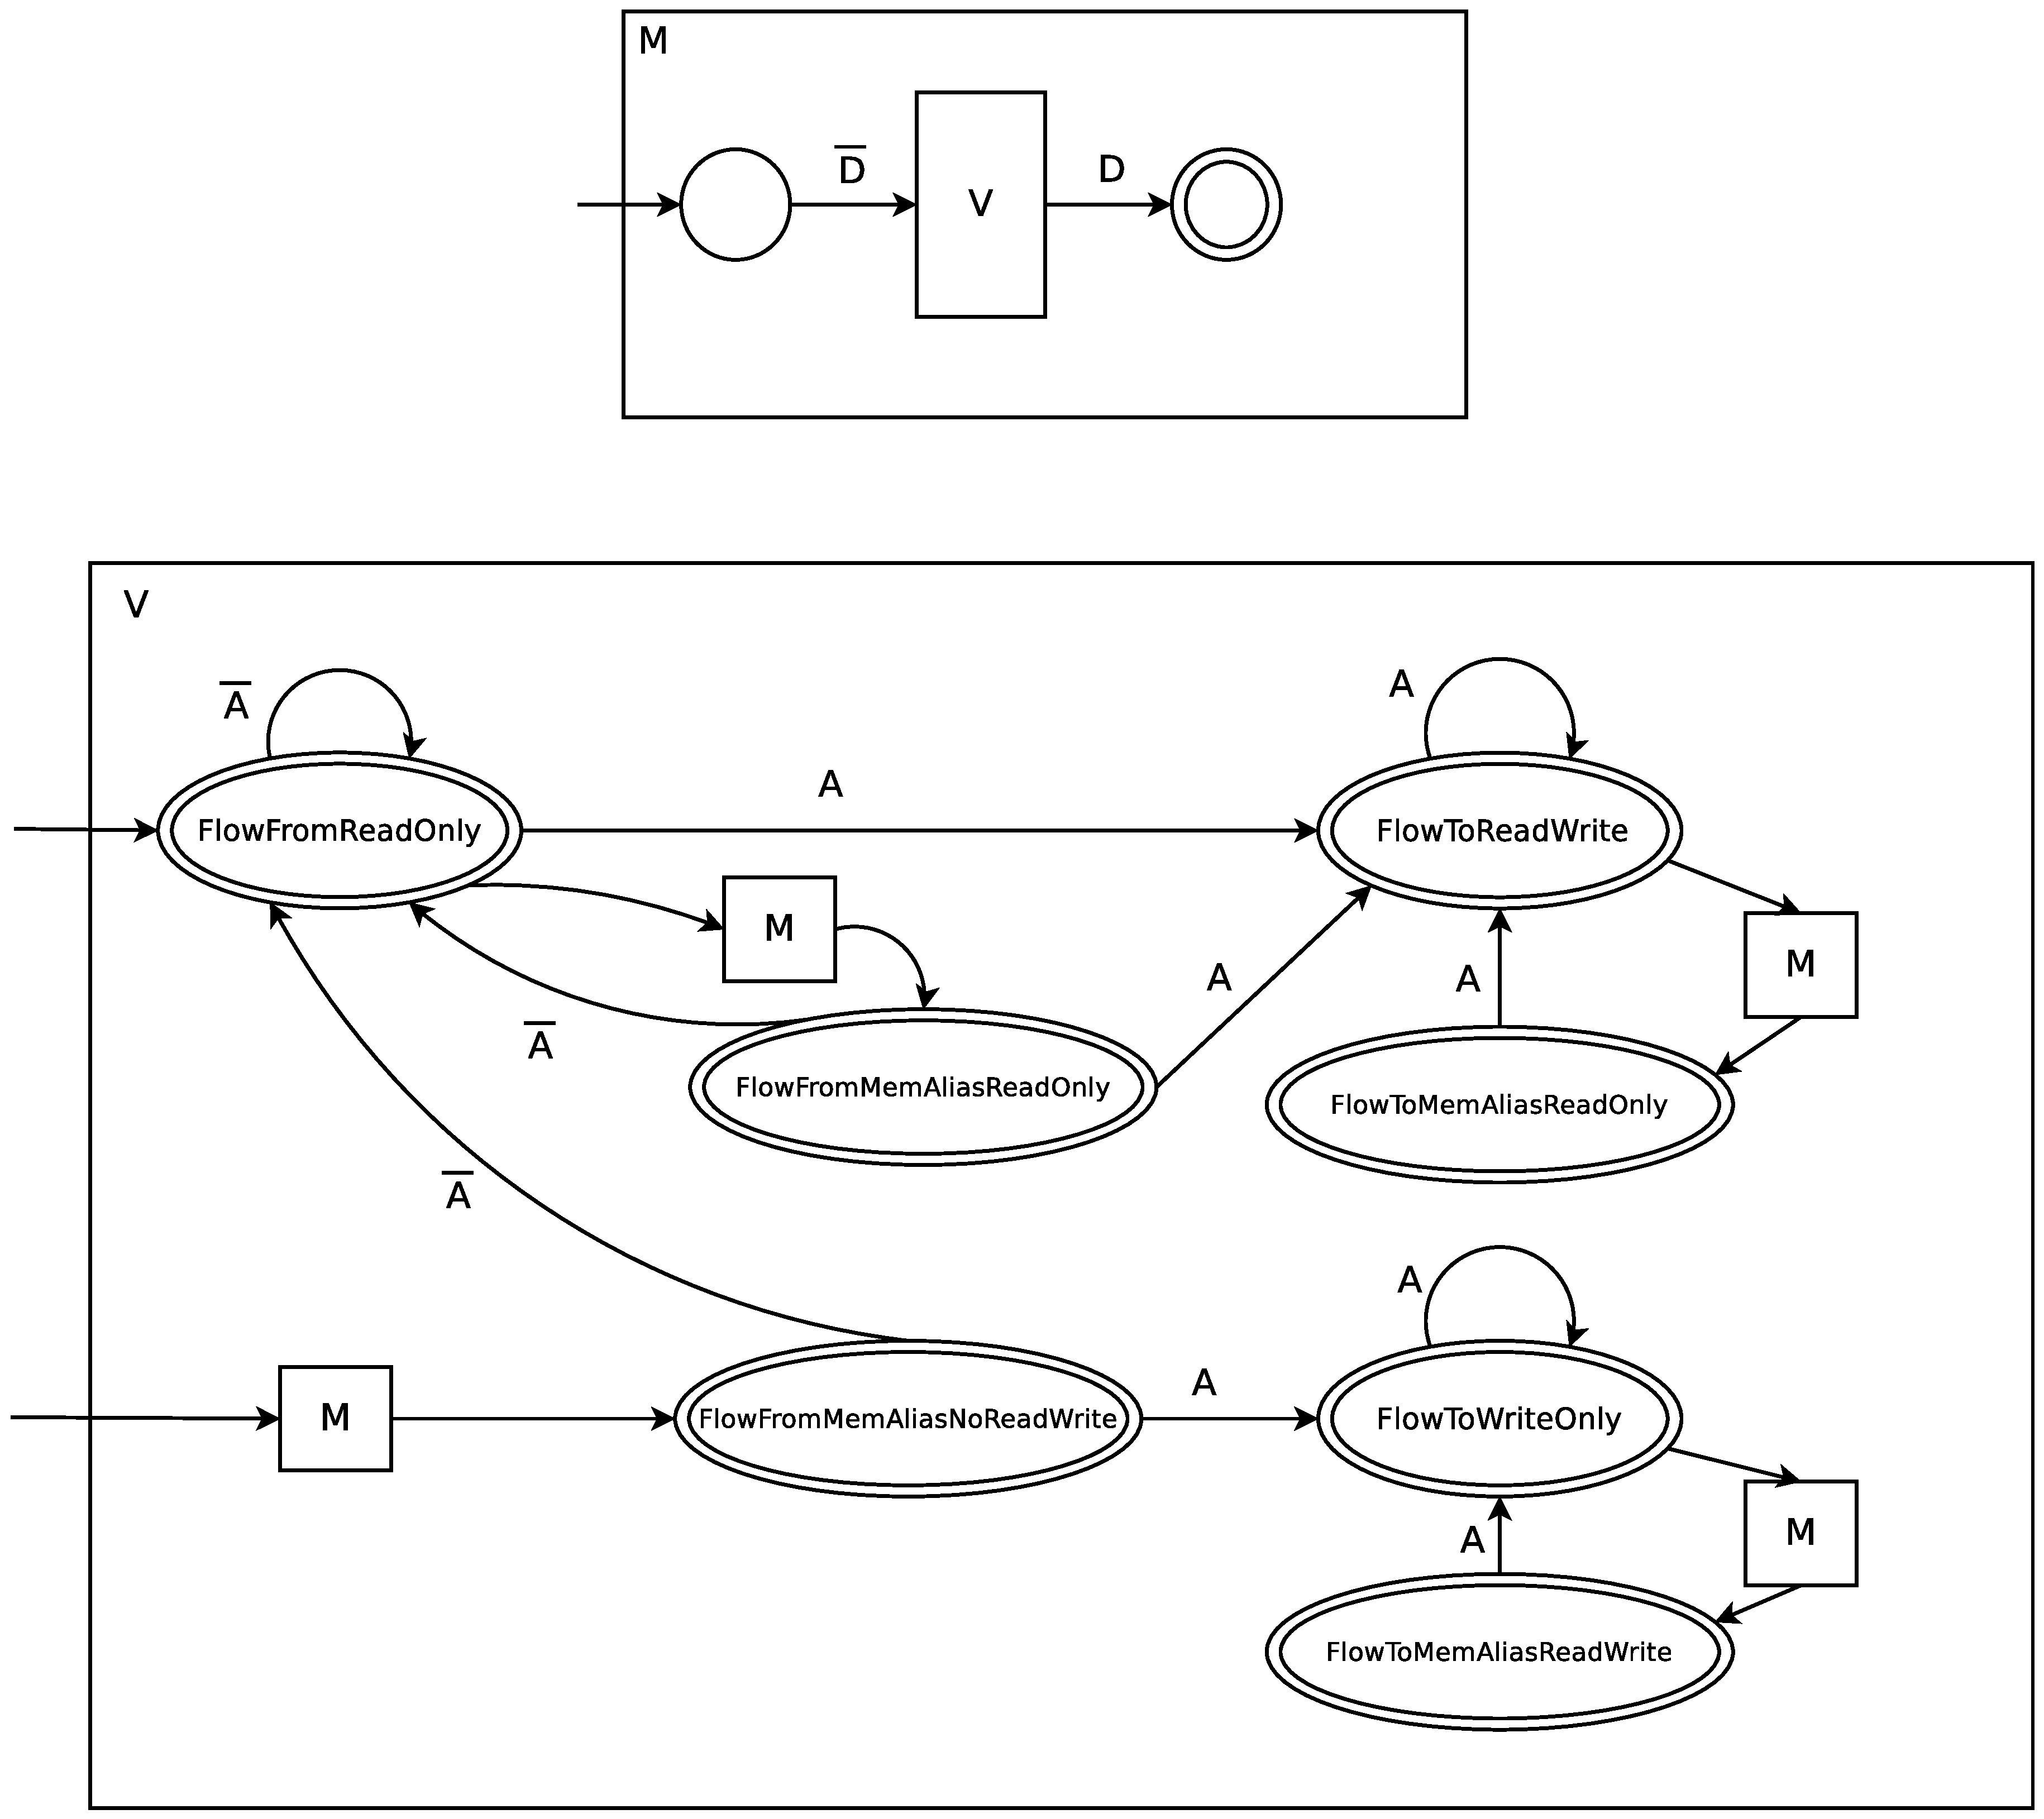
\includegraphics[width=350pt]{FSM2.eps}
  \caption{Hierarchical State Machine used in cfl-anders-aa.\label{fsm2} }
\end{figure}

\subsection{Node Attributes}\label{attribute}

Certain aspects in LLVM IR cannot be properly encoded into CFLGraph:
\begin{itemize}
  \item LLVM allows casts between pointers and integers, but CFLGraph only
    contains pointers as its nodes.
  \item LLVM module may contain global variables, which do no belong to any
    function and thus not modeled by CFLGraph.
  \item LLVM module may contain declared but not defined functions. CFLGraph has
    no way of knowing what their side-effects they have and therefore must
    assume that they can write anything to any memory location they get access
    to. 
\end{itemize}

To cope with the aforementioned language features, each node in CFLGraph is
associated with zero or more attributes. Attributes serve as ``escape hatches''
to our CFL Reachability algorithm: when a client queries the alias relation
between pointer $a$ and $b$, if either of them gets tagged with one or more 
attributes, the alias analysis will skip looking up their CFL reachability
lookup and
yield a response directly according to figure~\ref{attrs}. Attributes also
has the property that they get propagated ``downwards'': if $a$ gets tagged with
certain attributes, then everything that is transitively pointed to by $a$ also
gets tagged with the same set of attributes.

There are five different attributes: \emph{AttrEscaped}, \emph{AttrCaller},
\emph{AttrGlobal}, \emph{AttrArgument}, and \emph{AttrUnknown}. Here is a brief
explanation of their meaning:
\begin{itemize}
  \item Pointers that are allocated locally but somehow assigned to another value not
    modeled by the analysis get tagged with the \emph{AttrEscaped} attributes.
    Pointers that are casted into integers, or pointers that are used as actual
    parameters of some opaque function call, all fall into this category.
  \item Formal parameters of the current function get tagged with
    \emph{AttrArgument}. Values pointed to by those parameters get tagged with
    \emph{AttrCaller}.
  \item Global values themselves get tagged with \emph{AttrGlobal}.
  \item Any values that come from an unresolvable source (e.g.\ fabricated from
    integers, or loaded from opaque memory) are all tagged with
    \emph{AttrUnknown}. 
\end{itemize}

\begin{figure}\label{attrs}
\centering
\begin{tabular}{c|cccccc}
                       & \textbf{No Attributes} & \textbf{AttrEscaped} & \textbf{AttrGlobal} & \textbf{AttrArgument} & \textbf{AttrCaller} & \textbf{AttrUnknown} \\ \hline
\textbf{No Attributes} & CFL lookup             & CFL lookup           & NoAlias             & NoAlias             & NoAlias               & NoAlias              \\
\textbf{AttrEscaped}   & CFL lookup             & CFL lookup           & NoAlias            & NoAlias             & MayAlias               & MayAlias             \\
\textbf{AttrGlobal}    & NoAlias                & NoAlias              & MayAlias            & MayAlias            & MayAlias              & MayAlias             \\
\textbf{AttrArgument}  & NoAlias                & NoAlias              & MayAlias            & MayAlias            & MayAlias              & MayAlias             \\
\textbf{AttrCaller}    & NoAlias                & MayAlias             & MayAlias            & MayAlias            & MayAlias              & MayAlias             \\
\textbf{AttrUnknown}   & NoAlias                & MayAlias             & MayAlias            & MayAlias            & MayAlias              & MayAlias            
\end{tabular}
\caption{Rules for attribute handling. Rows represent the attributes of one
  pointer, and columns represent the attributes of another pointer. Each cell
  represents what response the analysis should return according to the
  attributes of the two given pointers. If there are more than one attributes
  for each pointer, combinations that lead to \emph{MayAlias} are prioritized
  over those that lead to \emph{NoAlias}. }
\end{figure}

\subsection{Interprocedural Analysis}\label{interproc}

The algorithm described in Section~\ref{steens} and Section~\ref{anders} both
work intraprocedurally. This section demonstrates how to extend those algorithms
to work in an interprocedural setting.

In general, there are two distinct approach to perform interprocedural analysis:
the top-down approach and the bottom-up approach. A top-down approach analyzes a
function \emph{before} it finishes analyzing all of its callee, while
bottom-up approach (a.k.a.\ summary-based approach) analyzes a function \emph{only
after} it finishes analyzing all of its callees. Top-down approaches are
generally more precise than bottom-up approaches, since when analyzing the
callees the analysis can put them in a known context. In contrast, in a
bottom-up approach functions
must be examined independently and out-of-context, where we
have zero information on the state of the memory, the arguments, the global
values, or anything else external to the function. To carry out the analysis
conservative assumptions have to be made about those external states. In
exchange for the potential loss of precision, we get better scalability: each
function only needs to be analyzed once, and the analysis result we obtain for
each function is highly reusable and can be applied to anywhere the function is
called.

Both cfl-aa passes use a bottom-up approach to look beyond function boundaries.
Each function gets analyzed independently and intraprocedurally at first, and we store the
externally visible effects of the function into a \emph{function summary}. The format
of those summaries is listed in figure~\ref{summary}. Subsequently, we
\emph{instantiate} each summary at each callsite of the corresponding function, replacing
\textbf{ReturnValue} with the right-hand side of the callsite, 
replacing \textbf{Parameter}$(i)$ with the $i$-th actual parameter of the
callsite, and tagging the return value and the parameters with the right set of
attributes. Finally, we incorporate the instatiated summary into the caller's
CFLGraph, and now the analysis can proceed as usual. In other words, the
interprocedural part of the anlysis is handled entirely at the CFLGraph
construction phase. The CFL Reachability computation is completely oblivious of
the function summaries, and therefore we do not need to make any change to it
for the interprocedural analysis to work.  

\begin{figure}[!ht]
  \begin{eqnarray*}
    \textit{FunctionSummary} & ::= & \textit{ExternallyVisibleEffect}^{*} \\
    \textit{ExternallyVisibleEffect} & ::= & \textit{InterfaceValue} = \textit{InterfaceValue}^\prime \\
                            & |   & \textit{InterfaceValue} \gets \textit{Attribute} \\
    \textit{InterfaceValue}  & ::= & \textbf{ReturnValue} \\
                    & |   & \textbf{Parameter}(i) \\
                    & |   & *\textit{InterfaceValue}^\prime \\
    \textit{Attribute}  & ::= & \textbf{AttrEscaped} \\
                    & |   & \textbf{AttrGlobal}  \\
                    & |   & \textbf{AttrUnknown}  
  \end{eqnarray*}
  \caption{Syntax of function summary\label{summary}}
\end{figure}

\section{Evaluation}\label{evaluation}

In this section, we evaluate both cfl-steens-aa and cfl-anders-aa using all
C/C++ programs in SPEC2006 benchmark. Souce codes of the test programs were first compiled
into LLVM bitcode file separately with optimization level 0, and then linked
together into a single bitcode file before any analysis gets
performed. The experiments were performed on a Ubuntu 14.04 environment, with Core i5 4330M as
the CPU and 8GB of RAM.\ Native gcc toolchain version on the system was 5.3.0.
The llvm and clang trunk revision used for the experiments is r278855.

\subsection{Alias Responses}

In the first set of experiments, we use the \textbf{-aa-eval} pass to query the
pairwise alias relations in the input bitcode, and count the percentage of
\emph{MayAlias} responses we get from each alias analysis under test. More
precise analyses tend to generate less \emph{MayAlias} responses, so lower
percentage is better. We test five different alias analysis settings:
\begin{itemize}
\item[-] Using basicaa alone
\item[-] Using cfl-steens-aa alone (referred to as ``steens'' for short)
\item[-] Using cfl-anders-aa alone (referred to as ``anders'' for short)
\item[-] Using basicaa combined with cfl-steens-aa (referred to as
  ``basicsteens'' for short)
\item[-] Using basicaa combined with cfl-anders-aa (referred to as
  ``basicanders'' for short)
\end{itemize}

The result can be found in figure~\ref{fig:alias_O0}\footnote{Cfl-anders-aa did not terminate for
  perlbench and gcc in 30 minutes. As a result corresponding data were not shown in the graph.}. For most of the
benchmarks, we can see that running cfl-steens-aa or cfl-anders-aa alone yields
worse result than running basicaa alone. One explanation is that basicaa has
been taught to handle far more cases than those cfl-aas do, including queries
that contain global values and \texttt{getelementptr}s. As a result, both
cfl-aas should not be used as a replacement of basicaa.

Putting cfl-aas behind basicaa, as figure~\ref{fig:alias_O0} suggests, behaves
consistently better than running basicaa alone. In some of the benchmarks (e.g.\
hmmer and omnetpp), the precision gain is rather significant. Benchmarks on
which the precision gains are small (e.g.\ bzip2 and sjeng) tend to use
structs and arrays extensively, and currently neither version of cfl-aa can handle
them in a precise manner.

\begin{figure}
  \centering
  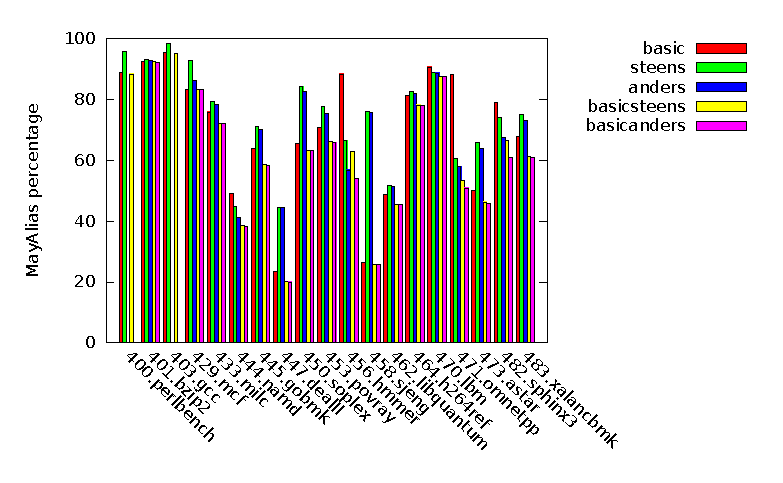
\includegraphics[width=\linewidth]{result/alias/aliasO0.eps}
  \caption{Percentage of may-alias responses (running on unoptimized bitcodes)\label{fig:alias_O0}}
\end{figure}

We also performed the same set of experiments after running \textbf{-mem2reg} on
the input program, as \textbf{-mem2reg} is able to remove a large amount of
unnecessary stack allocation and can reveal the program's memory-related
behaviors. Results are shown in
figure~\ref{fig:alias_Mem2reg}. Under this
scenerio, the precision gap between baiscaa and both versions of cfl-aas becomes
even bigger, but we do see that there are still times when running basicaa together
with cfl-aas could give basicaa a large precision boost.

\begin{figure}
  \centering
  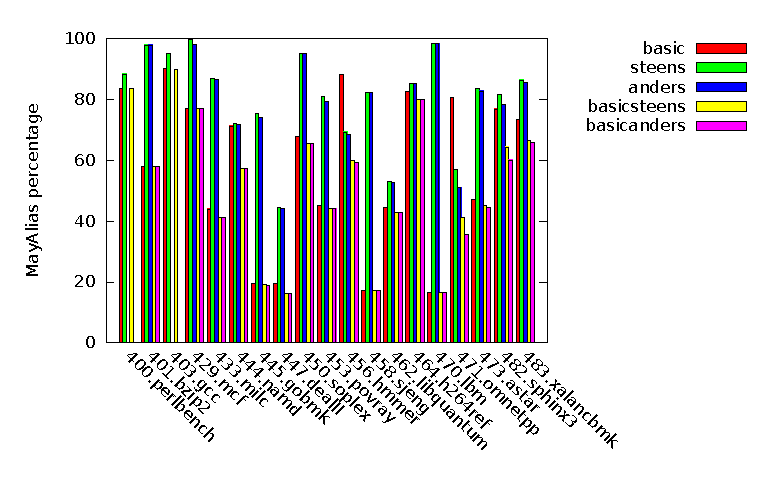
\includegraphics[width=\linewidth]{result/alias/aliasMem2reg.eps}
  \caption{Percentage of may-alias responses (running after \textbf{-mem2reg})\label{fig:alias_Mem2reg}}
\end{figure}

Figure~\ref{fig:aliasTime_O0} and figure~\ref{fig:aliasTime_Mem2reg} present the
running time for the two sets of experiments (lower is better). Data were
collected using a release build of llvm and clang. From the plot we can see that if
we take basicaa as a baseline, standalone cfl-steens-aa almost always runs
significantly faster, and standalone cfl-anders-aa usually runs noticeably
faster. It shows that basicaa is indeed a highly sophisticated analysis that can
do much more than both cfl-aas could handle\footnote{However, one important
  thing to point out here is that basicaa is a demand-driven analysis, and the
  performance numbers here were obtained by exhaustive alias pair queries. In
  practice, since clients rarely behave this way, we would expect the cost of
  basicaa to go down while the cost of both cfl-aas remains. }. When we put cfl-steens-aa behind
basicaa, normally we do not see much performance degradation except for a few
benchmarks. Running cfl-anders-aa with basicaa lead to a big slowdown, and if we
also consider the precision numbers from figure~\ref{fig:alias_O0} and
figure~\ref{fig:alias_Mem2reg}, this combination is simply not worth  not worth
to use. 

\begin{figure}
  \centering
  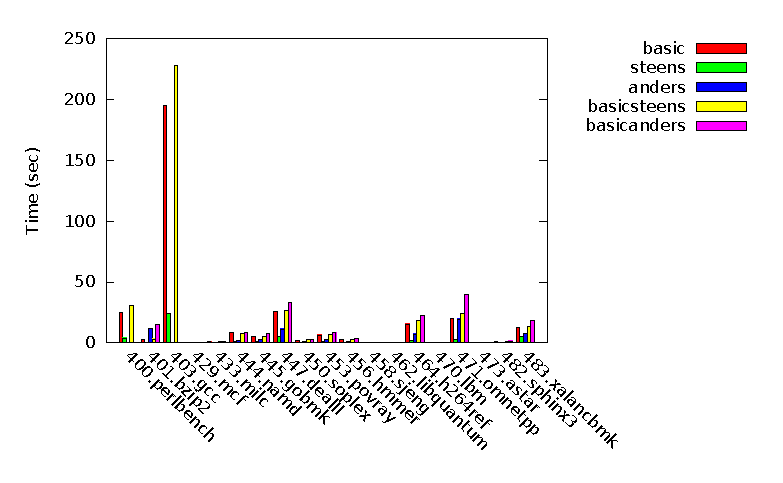
\includegraphics[width=\linewidth]{result/time/timeO0.eps}
  \caption{Analysis time (running on unoptimized bitcodes)\label{fig:aliasTime_O0}}
\end{figure}

\begin{figure}
  \centering
  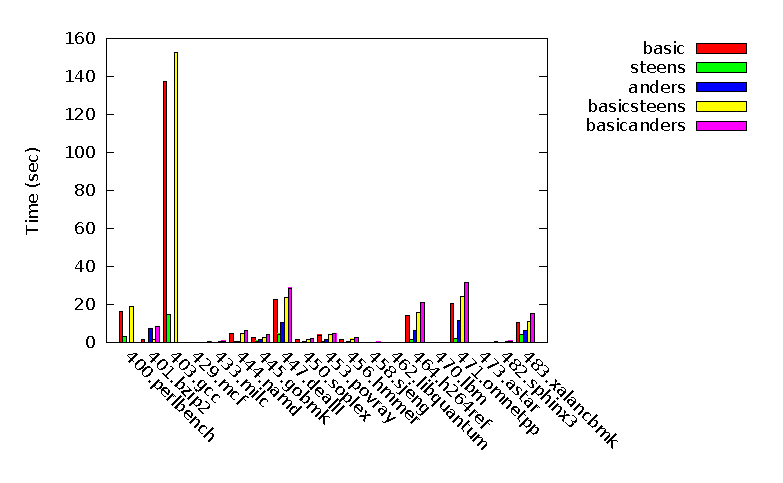
\includegraphics[width=\linewidth]{result/time/timeMem2reg.eps}
  \caption{Analysis time (running after \textbf{-mem2reg})\label{fig:aliasTime_Mem2reg}}
\end{figure}

\subsection{Impact to the clients}

In this section we evaluate cfl-aa by feeding their results to two optimization passes: loop invariant code motion
and global value numbering. Compared with the \textbf{-aa-eval} pass, licm and
gvn are more realistic clients and therefore can give us a better idea of
cfl-aa's utility in practice. All statistics here were collected by building LLVM with assertions, adding
-stats to the command line arguments, and then parsing the output. 

The first client we investigated is the licm pass. Measurement collected for
this client is the number of instructions hoisted out of the loop. Results are
shown in table~\ref{licm}. The second client we picked is the gvn pass\footnote{Technically
speaking, gvn does not use \texttt{AliasAnalysis} directly. But it heavily
relies on \texttt{MemoryDependenceAnalysis}, which in turn depends on
\texttt{AliasAnalysis}.}. Here we collected the number of instructions removed
by gvn, plus the number of instructions PRE'd by gvn, as both numbers
contributes to the quality of the optimization. The gvn results are shown in table~\ref{gvn}

We observe two trends in the dataset: first, cfl-steens-aa and cfl-anders-aa,
when used along with basicaa, consistently help to improve the effectiveness of
the clients. Second, when comparing the column of \emph{basicsteens} and \emph{basicanders}, we do not see
improvement at similar order of magnitude. 

\begin{table}[]
\centering
\caption{Numbers of instructions hoisted in licm (running on unoptimized bitcodes)}
\label{licm}
\begin{tabular}{@{}l|lllll@{}}
\toprule
               & basic & steens & anders & basicsteens & basicanders \\ \midrule
400.perlbench  & 3791  & 915    & -      & 3969        & -           \\
401.bzip2      & 1096  & 2546   & 2673   & 2901        & 3010        \\
403.gcc        & 19145 & 3739   & -      & 19788       & -           \\
429.mcf        & 169   & 97     & 150    & 217         & 217         \\
433.milc       & 4811  & 2743   & 2830   & 4833        & 4833        \\
444.namd       & 8511  & 3185   & 4390   & 8713        & 9287        \\
445.gobmk      & 9049  & 4557   & 4597   & 10620       & 10634       \\
447.dealII     & 48472 & 21577  & 21624  & 48484       & 48484       \\
450.soplex     & 7618  & 5166   & 5472   & 7642        & 7644        \\
453.povray     & 11822 & 6289   & 6508   & 12061       & 12153       \\
456.hmmer      & 5911  & 5158   & 5783   & 9400        & 9923        \\
458.sjeng      & 969   & 637    & 637    & 1109        & 1123        \\
462.libquantum & 1204  & 528    & 528    & 1228        & 1228        \\
464.h264ref    & 17589 & 19089  & 20978  & 28267       & 29563       \\
470.lbm        & 148   & 432    & 467    & 520         & 520         \\
471.omnetpp    & 1947  & 975    & 984    & 1954        & 1954        \\
473.astar      & 926   & 613    & 661    & 930         & 978         \\
482.sphinx3    & 3758  & 1637   & 1819   & 4156        & 4191        \\
483.xalancbmk  & 14631 & 8832   & 9071   & 14652       & 14658       \\ \bottomrule
\end{tabular}
\end{table}

\begin{table}[]
\centering
\caption{Number of instructions removed or PRE'd in gvn (running on unoptimized bitcodes)}
\label{gvn}
\begin{tabular}{@{}llllll@{}}
\toprule
               & basic  & steens & anders & basicsteens & basicanders \\ \midrule
400.perlbench  & 100135 & 79323  & -      & 100861      & -           \\
401.bzip2      & 9465   & 7931   & 9062   & 9864        & 9869        \\
403.gcc        & 300212 & 249682 & -      & 301410      & -           \\
429.mcf        & 1431   & 957    & 1387   & 1456        & 1467        \\
433.milc       & 13040  & 11990  & 12531  & 13232       & 13267       \\
444.namd       & 34181  & 31494  & 34510  & 35026       & 35030       \\
445.gobmk      & 75309  & 71925  & 72263  & 76717       & 76721       \\
447.dealII     & 165369 & 161826 & 164245 & 165634      & 165642      \\
450.soplex     & 26594  & 25786  & 27281  & 27206       & 27715       \\
453.povray     & 72402  & 66833  & 69825  & 73430       & 73487       \\
456.hmmer      & 30951  & 32796  & 34440  & 35117       & 35963       \\
458.sjeng      & 9734   & 7552   & 7610   & 9903        & 9908        \\
462.libquantum & 3299   & 3123   & 3123   & 3284        & 3284        \\
464.h264ref    & 64530  & 55566  & 59183  & 68659       & 69545       \\
470.lbm        & 2335   & 2712   & 2727   & 2730        & 2730        \\
471.omnetpp    & 22856  & 21409  & 22166  & 22859       & 22860       \\
473.astar      & 3626   & 3334   & 3491   & 3715        & 3789        \\
482.sphinx3    & 15621  & 14276  & 15553  & 16190       & 16302       \\
483.xalancbmk  & 193876 & 184509 & 191352 & 194205      & 194289      \\ \bottomrule
\end{tabular}
\end{table}

\section{Limitation}\label{limitation}

A properly functional alias analysis pass, just like many other analysis passes,
requires a large amount of tuning to work properly. Cfl-steens-aa and
cfl-anders-aa are no exception to this rule. In this section, we try to
summarize the shortcomings of the existing solution, and suggest ways to patch
or alleviate those problems in the future.

\paragraph{Cfl-anders-aa is slow} 

As shown in the evaluation section, cfl-anders-aa takes a long time to run, and
in some cases it even fails to terminate within a reasonable amount of time.
This is due to the lack of bug hunting and performance tuning: compared with cfl-steens-aa,
which has been curated by various developers for almost a year, cfl-anders-aa
was a one-man work created weeks
ago. As an inclusion-based context-sensitive analysis, cfl-anders-aa
inherently has higher computation cost, and therefore it heavily relies on
various form of optimizations~\cite{Hardekopf:2007}\cite{Hardekopf:2007_2}, as
well as performing demand-driven style calculations~\cite{Zheng:2008}, to boost its scalability. Currently none of those
optimizations get implemented, as at this early stage we choosed to prioritize
correctness over performance. Hopefully as cfl-anders-aa matures, those
optimizations can be added on top of the existing prototype.

\paragraph{Cfl-aa is field-insensitive}

Currently both versions of cfl-aa treats structs as a giant data blob, and do
not try to differentiate between different fields inside the same struct.
However, it is usually the case that if a struct contains more than one pointer
field, those fields tend to point to different locations. Collapsing structs
causes a great loss in terms of precision, and it may be one of the reason
why standalone cfl-aas get vastly outperformed by basicaa in terms of precision in the
evaluation section.

There has been some efforts spent on adding field sensitivity to cfl-anders-aa:
CFLGraph has been made field-offset aware, and the CFL Reachability propagation
logic already gets the ability to perform offset arithmetics. However, to
support field sensitivity at the interprocedural level, we need to adjust the
format of alias summaries and incorporate field offset as part of
\emph{ExternallyVisibleEffect}. This is the only issue left to be addressed
before we can put cfl-anders-aa into a full field-sensitive mode. 

On the other hand, no work was done to add field sensitivity support to
cfl-steens-aa. The decision to prioritize field-sensitive cfl-anders-aa over
field-sensitive cfl-steens-aa was made under the original hypothesis that
field-sensitivity may be less helpful to cfl-steens-aa due to its
unification-based nature. Given the evaluation numbers, it might be worth
reconsidering the validity of the hypothesis and add field-sensitive
cfl-steens-aa into our short-term goal.

\paragraph{Interprocedural analysis is imprecise for recursive calls}

In Section~\ref{interproc}, we mentioned that both cfl-aa passes analyze
functions in a bottom-up order: callees are examined before the callers. But if
we have potential recursive calls in the program (i.e.\ strongly connected
components in the call graph), a caller may be the callee of itself, on which
case we need additional rules to define the analysis order.

The current solution to break the recursive cycle is to pick a function on the
loop and conservatively treat it as an externally defined function (i.e.\ may write anything to
any memory location it has access to). Which function gets picked depends on which function
gets analyzed first, which in turn depends on what function the client queries
the alias analysis first.

Our current approach is sound, but may be imprecise since there is no guarantee that precision-critical
functions will not be treated conservatively. A more precise approach is to start the
analysis with the assumption that all functions have no side effect, then as we
discover more side effects by analyzing the body of each function, we propagate
the effects back to its callers. If the propagation adds even more side effects
to the caller, propagate them to the callers of the caller, and so on. We repeat the entire process until a fixpoint
is reached. This fixpoint strategy may be more costly than our current approach,
since we no longer have
the guarantee that each function gets analyzed only once: when there are
cycles on the call graph, functions on the call graph may be examined more than
once due to side effect propagation. Whether the precision gain is worth the
performance cost is another question to explore.

\paragraph{Cfl-aa lacks support for modref queries}

The \texttt{AliasAnalysis} interface in LLVM contains a wide range of APIs. Both
cfl-anders-aa and cfl-steens-aa only support the \texttt{alias()} queries.
However, \texttt{alias()} is not the only way clients interact with
AliasAnalysis. Another popular class of \texttt{AliasAnalysis} APIs are those
\texttt{getModRefInfo()} queries. The \texttt{getModRefInfo()} methods return
information about whether a given callsite (or a given callee) may read from or
write into certain memory locations. The information is very important to other
optimization passes that touches call or invoke instructions, because without
\texttt{getModRefInfo()} those passes would, say, refuse to move or delete
redundant function invocations, even if the alias analysis is 100\% confident
that the invocation is free of side effects.

There used to be naive modref supports in both CFL-based analyses: the
\texttt{getModRefInfo()} methods will just look into function summaries of the
alias analysis, and derive modref information accordingly. The support was
removed later, as we found that using alias analysis function summaries to derive modref information was
unsound: the summaries for alias analysis contain values of pointer-type
only, but a sound modref analysis must also consider reads/writes of non-pointer values. If a
function accesses a non-pointer value, the fact will not be reflected in the
alias summary, but it should be caught by the modref analysis.

A modref analysis may utilize alias summaries to figure out what memory locations
are accessed, but conceputally it is a separate analysis that has to consider a
wider range of values and therefore require more work than our naive implementations.

\paragraph{Collaboration with basicaa}

LLVM's basicaa pass is surprisingly efficient and precise, as shown in the
evaluation section. It is inherently demand-driven, handles a wider selection of values, and even has the
ability to decompose GEPs --- all of these nice features strongly suggest that
basicaa is not something that can be easily replaced by any other passes. The word ``basic'' in
basicaa does not mean ``naive'' or ``elementary''. Instead, it means
``essential'' and ``indispensable''. 

If basicaa is irreplaceable, then when it claims that two pointers are not
aliases, it might not be a good idea for other CFL-based passes to spend more
time just to rediscover
the same fact. A more detailed analysis of
basicaa's strength and weaknesses may be necessary, to provide better insights
into what aspects cfl-aas should be enhanced so that the enhancement does not
reimplement what basicaa can already do.  

\paragraph{Cfl-aa does not re-execute when function body gets changed}

Technically speaking, this is less a limitation of cfl-aa itself, and more of a
limitation of the LLVM alias analysis framework. However, the problem does have
a large impact to the utility of cfl-aas, so I think it is worth to be
pointed out here.

We we turn on cfl-anders-aa or cfl-steens-aa by specifying \texttt{-use-cfl-aa}
on the command line when optimization level is larger than 0, what the pass
manager will do is to put cfl-anders-aa or cfl-steens-aa at the front of the
pass pipeline, run it once, and never re-execute it afterwards. What happens
then is that the alias summaries generated by cfl-aas quickly becomes outdated after
several transformation passes take effects. Those transformation passes could
potentially add values to or remove values from the function body, and to stay sound cfl-aas have to
conservatively return \emph{MayAlias} if one or more values in the aliasing
queries are not found in its summary. If a large amount of values in the
function are not there we cfl-aa was first executed, then we might not be able
to obtain useful responses. As a result, only thos transformation passes that are
scheduled ``early'' on the optimization pipeline enjoy the benefit of cfl-aas.
Passes that are scheduled ``late'' will behave almost the same, regardless
of whether cfl-aas are turned on or not.

It would be nice to have the pass manager periodically re-execute cfl-aas after certain
number of transformation passes, or to allow transformation passes
to explictly invalidate cfl-aa summaries such that they could get automatically
recomputed by cfl-aas.

\section{Conclusion}\label{conclusion}

In this article we discussed about the design and implementation of two
flow-insensitive, context-sensitive LLVM alias analysis passes. Both passes are based on a CFL Reachability solver with
different tradeoff between precision and performance. We evaluated those passes
using real-world clients and benchmarks, and proposed various ways to improve upon the current implementations.

The original title of the project is called \emph{Better Alias Analysis By
  Default}. Based on the evaluation numbers, basicaa+cfl-steens-aa might be a promising
candidate to set as the default alias analysis for LLVM, if the re-execution
issue mentioned in Section~\ref{limitation} can be properly addressed.  

\section*{Acknowledgement}

Many thanks to my mentors George Burgess IV, who helped me get
started on the project and reviewed all of my patches, and Hal Finkel, who
provided me with access to high-performance platforms as well as valuable information
on testing and debugging.  

I would also like to show my gratitude to Daniel Berlin for sharing his ideas
and knowledge with me through email discussions.

Kudos to all other devs on phabricator who have reviewed my codes. 

\bibliography{reference}{}
\bibliographystyle{plain}
\end{document}
